% Slide 3 — Système de Motion Capture
\subsubsection{Système de Motion Capture}
\begin{frame}{Système de Motion Capture (OptiTrack)}
\begin{columns}[T]
  \begin{column}{0.55\textwidth}
    \begin{itemize}
      \item Suivi d'objets en temps réel par capture de mouvement.
      \item Utilise des caméras infrarouges et des marqueurs réfléchissants sur les robots.
      \item Le logiciel Motive calcule la pose (position et orientation) des objets (appelés \textit{Rigid Bodies}).
      \item Communication avec ROS 2 via le protocole VRPN pour une localisation précise.
    \end{itemize}
  \end{column}
  \begin{column}{0.45\textwidth}
    \begin{figure}
      \centering
      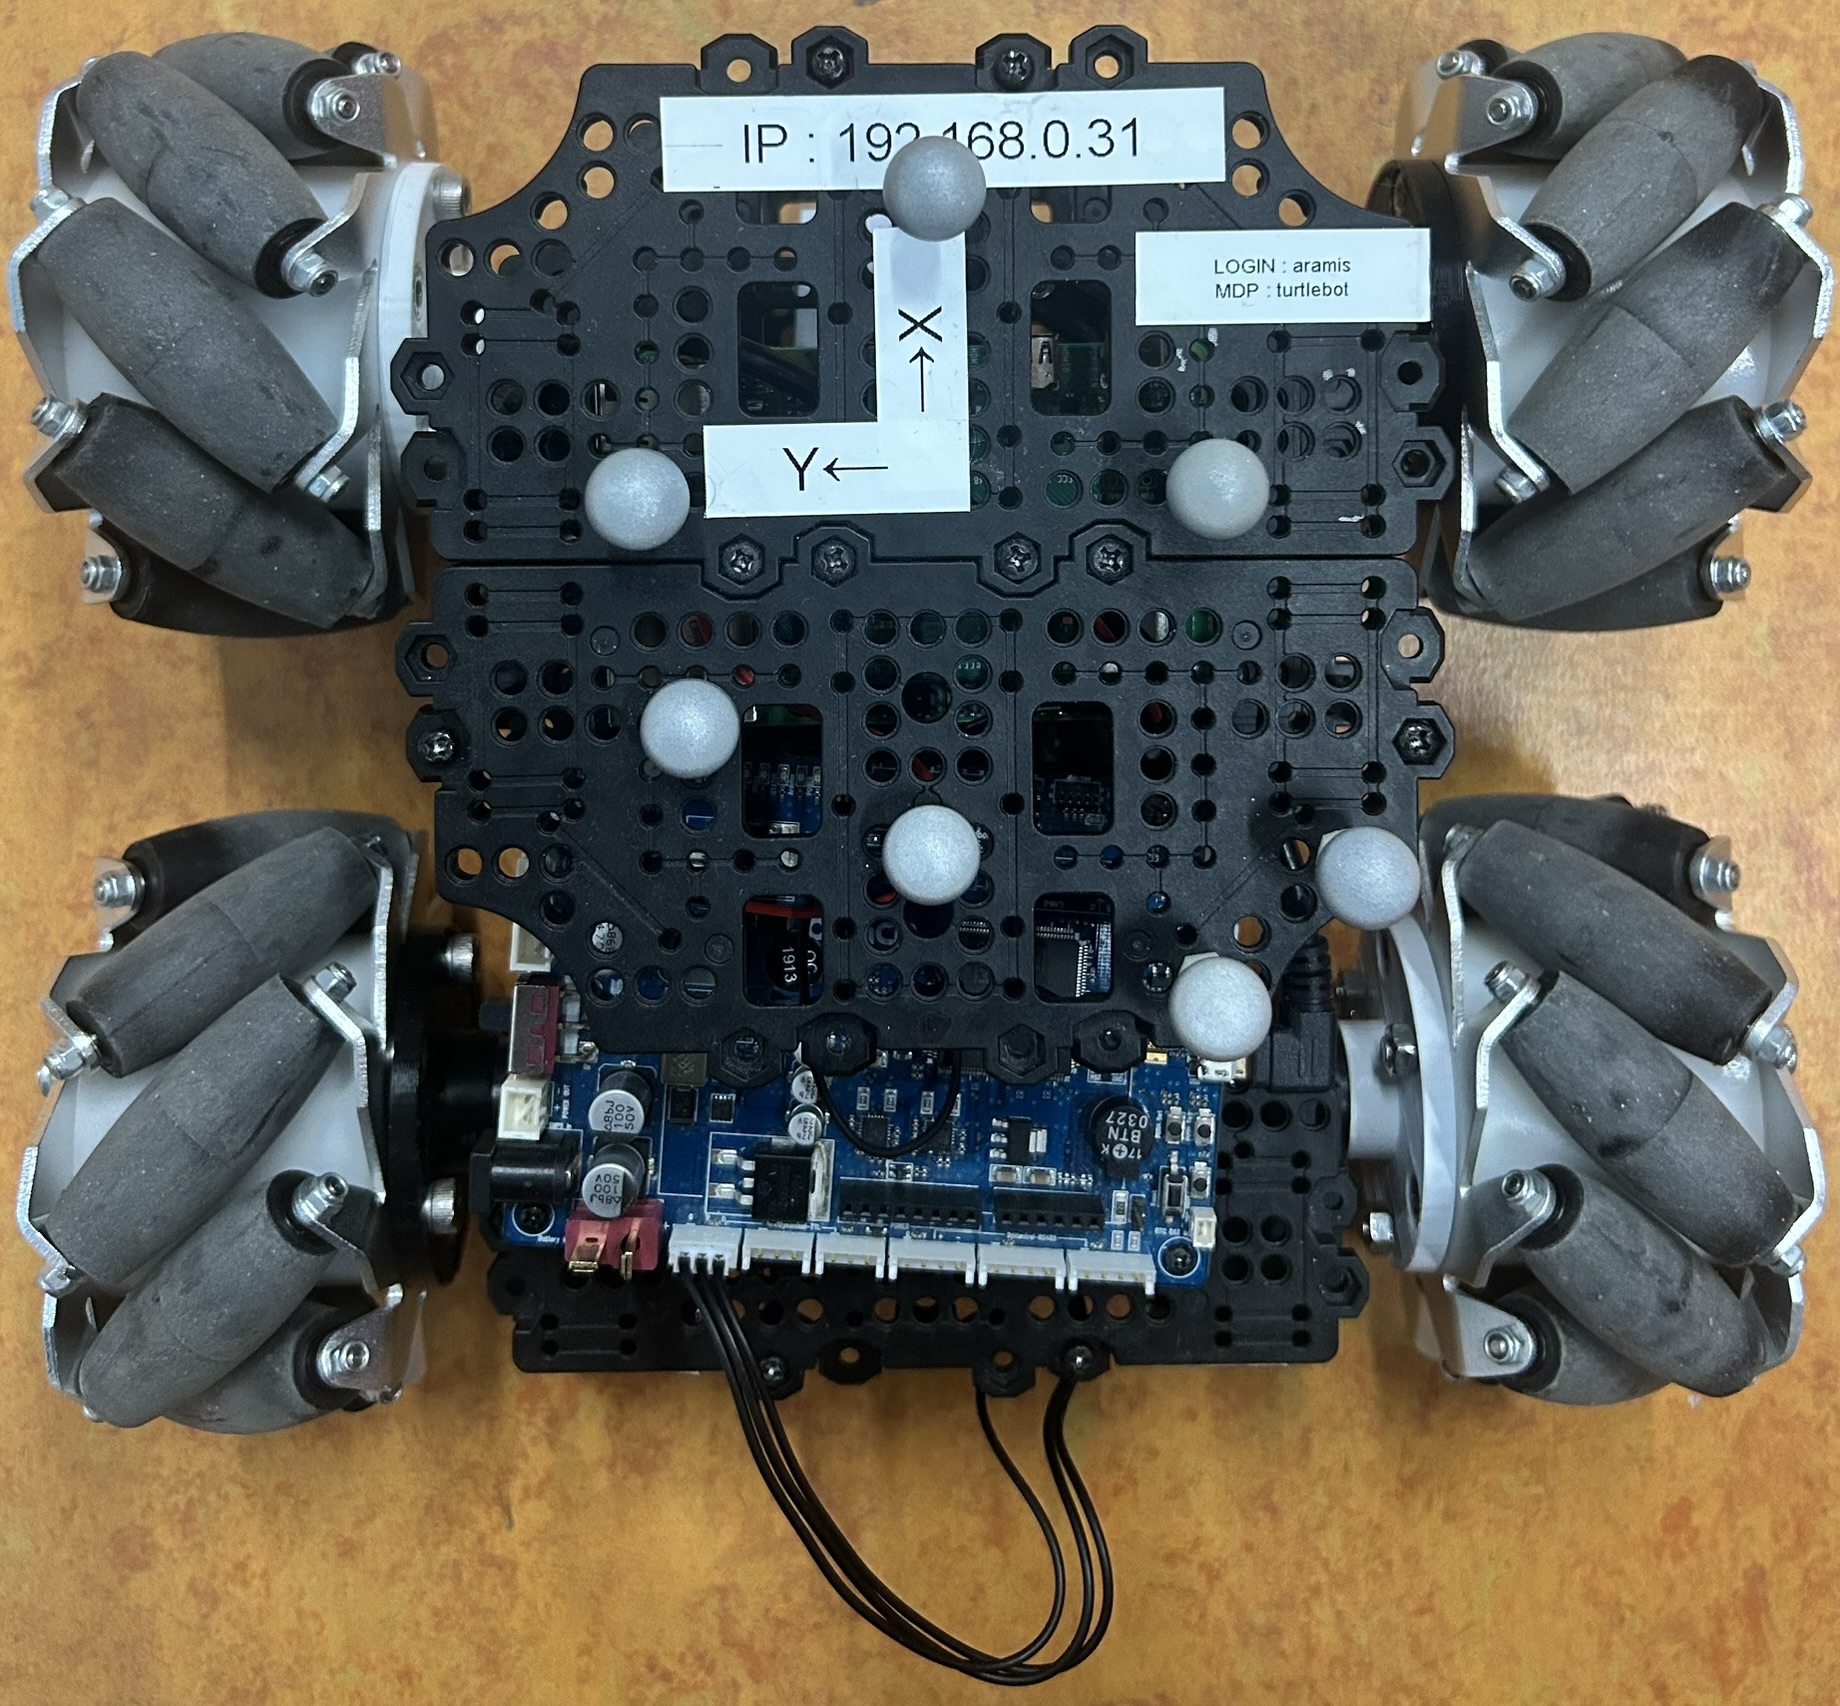
\includegraphics[width=0.48\textwidth]{5-Descriptions-realisations/outils/pic/billes.JPEG}
      \hfill
      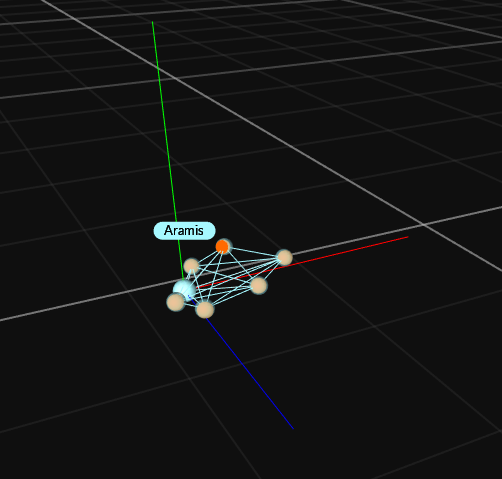
\includegraphics[width=0.48\textwidth]{5-Descriptions-realisations/outils/pic/aramis.PNG}
      \caption{Marqueurs sur un robot et son \textit{Rigid Body} dans Motive.}
    \end{figure}
  \end{column}
\end{columns}
\end{frame}
